% TODO: difference between intermediate and final output images?

\documentclass[11pt, english]{article}
\usepackage[a4paper, margin=2.5cm]{geometry}
\usepackage{graphicx} % Required for inserting images
\usepackage[useregional]{datetime2}
\usepackage{tabularx}

\begin{document}

\pagenumbering{gobble}% Remove page numbers (and reset to 1)
\thispagestyle{empty}
\begin{titlepage}
\begin{center}
  \centering
  
  \Huge \textbf{COMP9517 - Assignment 1} \\
  \vspace{5cm}
     
  \huge \textbf{Ryan McClue} \\
  (z5346008)
  \vspace{5cm}
    
  \today
\end{center}
\end{titlepage}

\section{Q1}
\section{Q2}
\section{Q3}
\section{Q4}
\begin{table}[ht]
\centering
\begin{tabularx}{\linewidth}{X|X|X|X|X}
Input Image & Histogram & Otsu Thresholding & Isodata Thresholding & Triangle Thresholding \\\hline
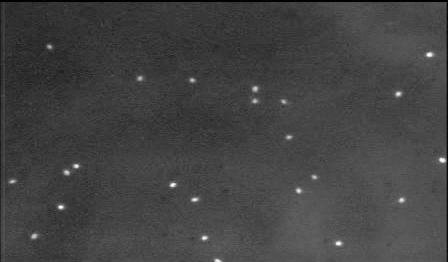
\includegraphics[width=0.18\textwidth]{Algae.png} & 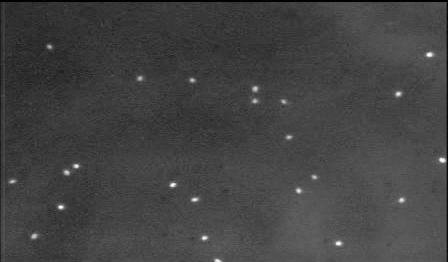
\includegraphics[width=0.18\textwidth]{Algae.png} & 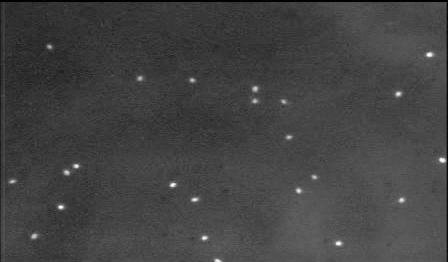
\includegraphics[width=0.18\textwidth]{Algae.png} & 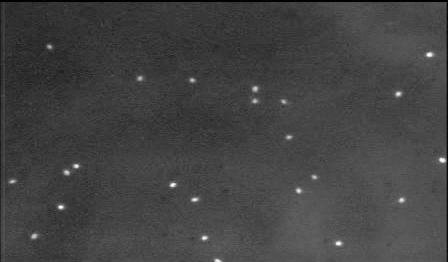
\includegraphics[width=0.18\textwidth]{Algae.png} & 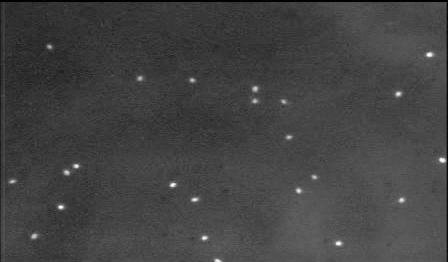
\includegraphics[width=0.18\textwidth]{Algae.png} \\
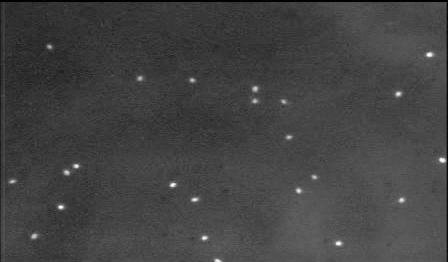
\includegraphics[width=0.18\textwidth]{Algae.png} & 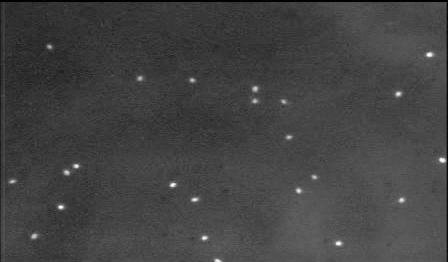
\includegraphics[width=0.18\textwidth]{Algae.png} & 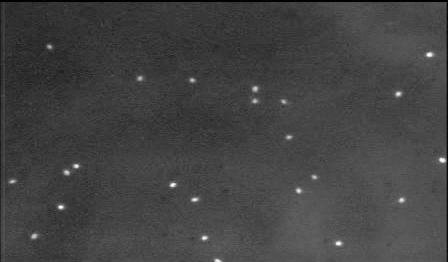
\includegraphics[width=0.18\textwidth]{Algae.png} & 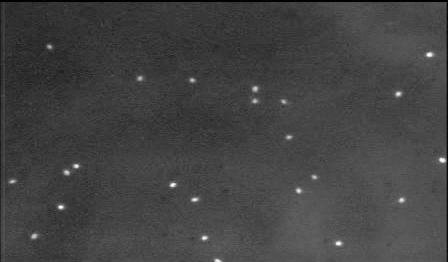
\includegraphics[width=0.18\textwidth]{Algae.png} & 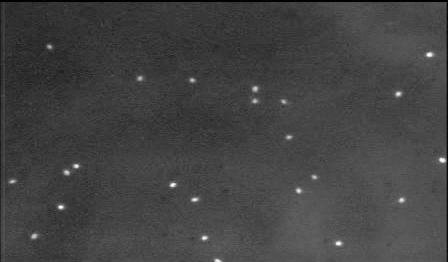
\includegraphics[width=0.18\textwidth]{Algae.png} \\

\end{tabularx}
\caption{An example table.}
\end{table}


\end{document}


% The report can be
% written in Word, LaTeX, or a similar text processor, but must be submitted as a PDF and
% include your name and zID on the first page. It must also show the sample input images
% and the intermediate and final output images obtained. No templates are provided, but
% the report must be no more than 5 pages (A4), and must be single column, use 11 points
% Times New Roman or similar font, and have 2.5 cm margins.

% In your report, discuss the differences in the results and provide explanations (based on the
% histograms or otherwise) why for some images one thresholding technique may work betterthan others, 
% while for other images it may be the other way around.
% Present some general guidelines for which thresholding techniques are best for which kinds of images.

% include an explanation of the approach you have taken to each of the tasks and your conclusion in the report in PDF format 
% just high-level algorithm aspect explanation 
